\documentclass[tikz,border=3mm]{standalone}

\usepackage{xcolor}
\colorlet{myred}{red!80!black}

\begin{document}
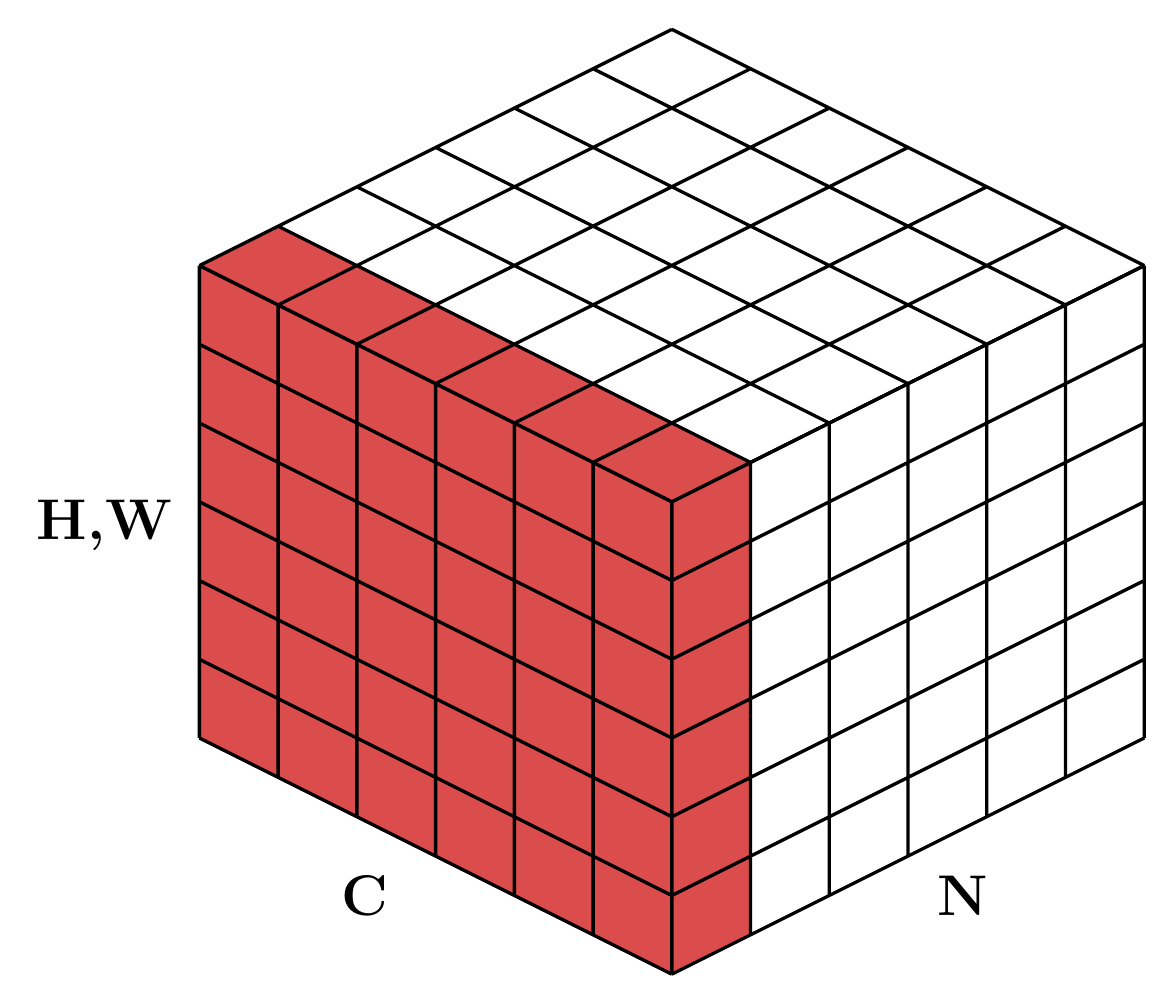
\begin{tikzpicture}

  % Grid with yslant=-0.5
  \fill[myred!70, yslant=-0.5] (0,0) rectangle (6,6);
  \draw[very thick,yslant=-0.5] (0,0) grid (6,6);
  
  % Grid with yslant=0.5
  \fill[myred!70, yslant=0.5] (6,-6) rectangle (7,0);
  \draw[very thick,yslant=0.5] (6,-6) grid (12,0);

  % Grid with yslant=0.5 and xslant=-1
  \fill[myred!70, yslant=0.5, xslant=-1] (6,0) rectangle (7,6);
  \draw[very thick,yslant=0.5,xslant=-1] (6,0) grid (12,6);

  \node at (-1.2,2.7) {\huge\textbf{H,W}};
  \node at (9.7,-2) {\huge\textbf{N}};
  \node at (2.1,-2) {\huge\textbf{C}};
\end{tikzpicture}
\end{document}
